\subsubsection{Pumps}

The starting and stopping of pumps are a significant cause of transient flows in pumping systems. Starting of a pump is usually controlled by keeping the discharge valve close until the pump reaches the rated speed and then slowly opening the valve. However sometimes pumps are started without using valves by controlling the speed electronically. Similarly pump shutdown may be assisted by valve closure or by external control. Another common source of pump transients is power failure, in this situation the speed of the pump is no longer controlled and is instead determined by the torque on the pump and the flow conditions.  

\paragraph{Shutdown}

The simplest way to shutdown a pump in a controlled manner is a reduction of the rotational speed, at a specified event time $t_e$, to zero at time $t_e + t_c$, where $t_c$ is stopping time. The rotational speed $N$ as a function of time $t$, as shown in figure \ref{fig:pump_shutdown}, is defined by the piecewise function
\begin{align}\label{pump_shutdown_function}
N(t) = 
\begin{cases} 
N_{steady}, &\text{if} \hspace{0.5cm} t \leq t_e \\
N_{steady} \left( 1 - \frac{t-t_e}{t_c} \right)^m, &\text{if} \hspace{0.5cm} t_e \leq t \leq t_e + t_c \\
0, &\text{if} \hspace{0.5cm} t \geq t_e + t_c. 
\end{cases}
\end{align}
The exponent $m > 0$ modifies the shape of the closure profile with $m=1$ corresponding to a linear profile. Changing the rotational speed alters both $n$ and $\theta$ in the pump resistance equation \eqref{pump_resistance} so that the resistance varies with time too. 

\begin{figure}
\centering
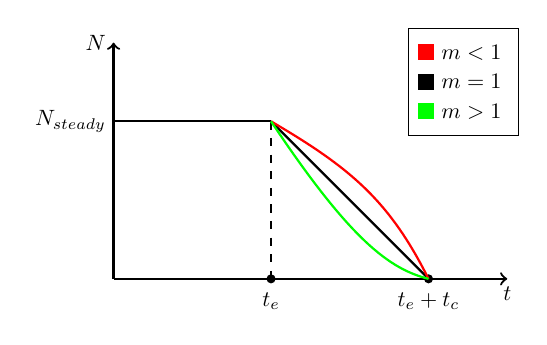
\begin{tikzpicture}[
	scale=1, 
	every node/.style={scale=0.8},
	greennode/.style={shape=rectangle, fill=green, draw=green, minimum size =0.01cm},
	rednode/.style={shape=rectangle, fill=red, draw=red, minimum size =0.01cm},
	blacknode/.style={shape=rectangle, fill=black, draw=black, minimum size =0.01cm},
] 
\draw[thick, ->] (0,0) -- (0,3);
\node[anchor=east] at (0,3) {$N$};
\draw[thick, ->] (0,0) -- (5,0);
\node[anchor=north] at (5,0) {$t$};
\node[anchor=north] at (2,-0.08) {$t_e$};
\draw[fill=black] (2,0) circle (0.05cm);
\node[anchor=north] at (4,-0.08) {$t_e + t_c$};
\draw[fill=black] (4,0) circle (0.05cm);
\node[anchor=east] at (0,2) {$N_{steady}$};
\draw[thick] (0,2) -- (2,2);
\draw[thick] (2,2) -- (4,0);
\draw[thick, dashed] (2,2) -- (2,0);
\draw[thick, red] (2,2) .. controls (3,1.414) and (3.5,1) .. (4,0);
\draw[thick, green] (2,2) .. controls (3,0.5) and (3.5,0.125) .. (4,0);

\matrix [draw,below left] at (current bounding box.north east) {
  \node [rednode,label=right: {$m < 1$}] {}; \\
  \node [blacknode,label=right: {$m = 1$}] {}; \\
  \node [greennode,label=right: {$m > 1$}] {}; \\
};
\end{tikzpicture} 
\caption{Pump shutdown. The rotational speed $N(t)$ goes from $N_{steady}$ at time $t_e$ to zero at time $t_e + t_c$, where $t_c$ is the time taken for the pump to stop. The exponent $m$ modifies the closure profile, as shown by the red and green curves.}
\label{fig:pump_shutdown}
\end{figure}

\paragraph{Startup}

The time varying function describing the startup of a pump, as shown in figure \ref{fig:pump_startup}, is very similar to the function describing a shutdown and is given by 

\begin{align}\label{pump_startup_function}
N(t) = 
\begin{cases} 
0, &\text{if} \hspace{0.5cm} t \leq t_e \\
N_{\infty} \left( \frac{t-t_e}{t_s} \right)^m, &\text{if} \hspace{0.5cm} t_e \leq t \leq t_e + t_s \\
N_{\infty}, &\text{if} \hspace{0.5cm} t \geq t_e + t_s, 
\end{cases}
\end{align}
where again $t_e$ is the event time, $t_s$ is startup time and $N_{\infty}$ is the pump speed once the startup procedure has been completed. The exponent $m > 0$ modifies the shape of the closure profile with $m=1$ corresponding to a linear profile. 


\begin{figure}
\centering
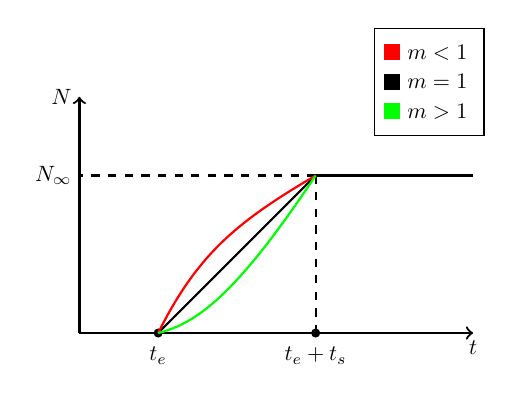
\begin{tikzpicture}[
	scale=1, 
	every node/.style={scale=0.8},
	greennode/.style={shape=rectangle, fill=green, draw=green, minimum size =0.01cm},
	rednode/.style={shape=rectangle, fill=red, draw=red, minimum size =0.01cm},
	blacknode/.style={shape=rectangle, fill=black, draw=black, minimum size =0.01cm},
] 
\draw[thick, ->] (0,0) -- (0,3);
\node[anchor=east] at (0,3) {$N$};
\draw[thick, ->] (0,0) -- (5,0);
\node[anchor=north] at (5,0) {$t$};
\node[anchor=north] at (1,-0.08) {$t_e$};
\draw[fill=black] (1,0) circle (0.05cm);
\node[anchor=north] at (3,-0.08) {$t_e + t_s$};
\draw[fill=black] (3,0) circle (0.05cm);
\node[anchor=east] at (0,2) {$N_{\infty}$};

\draw[thick] (3,2) -- (5,2);
\draw[thick] (1,0) -- (3,2);
\draw[thick, dashed] (3,2) -- (3,0);
\draw[thick, dashed] (3,2) -- (0,2);
\draw[thick, red] (1,0) .. controls (1.5,1) and (2,1.414)  .. (3,2);
\draw[thick, green] (1,0) .. controls (1.5,0.125) and (2,0.5) .. (3,2);

\matrix [draw,left] at (current bounding box.north east) {
  \node [rednode,label=right: {$m < 1$}] {}; \\
  \node [blacknode,label=right: {$m = 1$}] {}; \\
  \node [greennode,label=right: {$m > 1$}] {}; \\
};
\end{tikzpicture} 
\caption{Pump startup. The rotational speed $N(t)$ goes from zero at time $t_e$ to $N_{\infty}$ at time $t_e + t_s$, where $t_s$ is the time taken for the pump to startup. The exponent $m$ modifies the closure profile, as shown by the red and green curves.}
\label{fig:pump_startup}
\end{figure}

% \paragraph{General speed variation (piecewise linear)}

% \paragraph{Power failure}